%!TEX root =  main.tex
In this section we establish that SAP with strong dominance property is `regret equivalent' to an instance of MAB with side-information and the corresponding algorithm for MAB can be suitably imported to solve SAP efficiently.   
 \noindent
\begin{definition}[Regret Equivalence]
	Consider a SA-Poblem $\psi:=(K, P, c)$ and a bandit problem $\phi:=(N, (\nu_i)_{i \in [N]},G)$ with side-information graph $G$. We say that $\psi$ is regret-equivalent to $\phi$ if given a policy $\pi$ for $\psi$, one can come up with a policy $\pi^\prime$ that uses $\pi$, such that the regret of $\pi^\prime$ on any instance of $\phi$ is the same as the regret of $\pi$ on some corresponding instance of $\psi$, and vice versa. 
\end{definition}	
In the following we first consider SAP with $2$ sensors and then the general case with more than $2$ sensors. SAP with $2$ sensors is useful to draw comparison with the well studied apple tasting problem \cite{IC2000_AppleTasting_HelmboldLittlestoneLong} and understand role of the dominance property. 
\subsection{SAP with two sensors}
In SAP with two sensors, while action $1$ reveals no information about the loss values, under dominance property, action $2$ reveals (partial) information about the loss from both actions. To see this, let $I_t=2$. If predictions of sensors disagree, i.e., $\hat{Y}^1_t\neq\hat{Y}^2_t$, then  dominance property implies that only sensor $2$ is correct, i.e., $\hat{Y}^1_t \neq Y_t$ and $\hat{Y}^2_t=Y_t$. Hence $L_t(1)=1$ and $L_t(2)=c$. On the other hand, if predictions agree, i.e., $\hat{Y}^1_t = \hat{Y}^2_t$, then either predictions of both are correct or both are incorrect, and we can only infer that $L_t(2)-L_t(1)=c_1+c_2>0$. Thus, each time learner plays action $2$,  loss from both actions is known only when sensor output disagree, otherwise. 

\noindent
{\bf Apple tasting \cite{IC2000_AppleTasting_HelmboldLittlestoneLong}:} In this problem, a learner gets a sequence of apples some of which can be rotten. In each round, the learner can either accept or reject an apple and irrespective of his action, a penalty is incurred if the apple is rotten in that round. If an apple is rejected, learner do not get to observe its quality, and if accepted, the learner tastes the apple and knows its quality. In the latter case loss incurred is known, and the learner can also know the loss he would have incurred if he opted to reject it.  %Thus, each time the learner accepts an apple, he knows the penalty incurred for both the actions. However, no loss values is revealed if he rejects. 
The goal of the learner is to taste more good apples. 
A SAP with dominance property is thus a general version than the apple tasting problem as unlike in apple tasting problem loss value are revealed only in few instances.  We next show that SAP satisfying dominance property can be efficiently solved.  
%
%\begin{thm}
%	\label{thm:2SAPRegret}
%Assume dominance condition (\ref{eqn:DominanceCondition}) holds. Then SAP $\psi$ with $K=2$ is regret-equivalent to a stochastic $1$-armed bandit.
%\end{thm}
%%a_i\mathbb{E}[N_i(T)]$ where $\Delta_1= c- \min\{\gamma_1-\gamma_2,c\}$ and $\Delta_2= \gamma_1-\gamma_2- \min\{\gamma_1-\gamma_2,c\}$, which can also be expressed as $\Delta_1=\gamma_1 - \mathbb{E}[L(i^*)]$ and  $\Delta_2=\gamma_2+c - \mathbb{E}[L(i^*)]$, implying that the corresponding policy on the SAP also gives the same regret and vice versa. 
%The following corollary follow immediately from the regret equivalence. 
%\begin{proposition}[SAP regret lower bound]
%	Let $\pi$ be any policy on SAT with 2 sensors such that it pulls the suboptimal arm only sub polynomial many times, i.e., $\mathbb{E}[N_i(T)]=o(T^a)$ for all $a>0$ and $i\neq i^*$. Then,
%	\begin{equation}
%	\liminf_{T \rightarrow \infty} R^\psi_T(\pi)/\log T \geq \frac{|\gamma_1-\gamma_2-c|}{D(\hat{\gamma},\gamma^*)} \mbox{ where } \gamma^*=\min\{\gamma_1,\gamma_2+c\},  \hat{\gamma}=\max\{\gamma_1,\gamma_2+c\}
%	\end{equation}
%	and $D(\hat{\gamma},\gamma^*)$  is the KL-divergence between $\hat{\gamma}$ and $\gamma^*$.
%\end{proposition}
%
%\begin{proposition}[SAP regret upper bound]
%	Let $\pi^\prime$ denote a policy on a $1$-armed stochastic bandit where one arm has mean $\gamma_1-\gamma_2$ and the other gives fixed reward $c$. Then, the regret of a policy $g(\pi)$ for the SAT problem obtained according the mapping (\ref{eqn:1BanditToSAP}) is upper bounded as
%	\begin{equation}
%	R^\psi_T(g(\pi))\leq \frac{6\log T}{|\gamma_1-\gamma_2-c|} + |\gamma_1-\gamma_2-c|(1+\pi^2/3) 	\mbox{ when } \pi^\prime=\mbox{UCB1}. 
%	\end{equation}
%		\begin{equation}
%		R^\psi_T(g(\pi))\leq \frac{|\gamma_1-\gamma_2-c|\log T}{D(\hat{\gamma},\gamma^*)} + \mathcal{O}(\sqrt{\log T }) 	\mbox{ when } \pi^\prime=\mbox{KL-UCB}. 
%		\end{equation}
%\end{proposition}
\subsection{SAP with more than two actions}

\begin{wrapfigure}{r}{6cm}
	\centering
	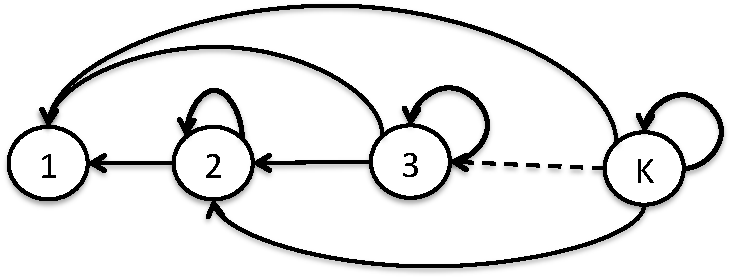
\includegraphics[scale=.4]{SideInfoGraph.pdf}
	\caption{Side observation graph $G_S$}
	\label{fig:SideObservationGraph]}
\end{wrapfigure} 
In SAP with two sensors, only action $2$ provides partial information about the loss of both actions. In the case with $K>2$ sensors, by playing an action $k$, partial information about the loss from actions $l<k$ can be inferred by recursively applying the dominance property to each pair of sensors.  Further, any information provided by action $k>2$ is contained in that provided by all actions $k^\prime\geq k$ as $H_t(k) \subseteq H_t(k^\prime)$. 

This information structure can be represented by a directed graph $G_S=(V,E)$, where $|V|=K$ and $E=\{(i,j): 1<i\leq j\leq K \}$. Note that $G_S$ has self loops for all nodes except for node $1$. The nodes in $G_S$ represents actions of in SAP and an edge $(i,j)\in E$ implies that actions $i$ provides information about action $j$. The side-observation graph for the SAP is shown in Figure (\ref{fig:SideObservationGraph]}).

We now have all the ingredients to relate SAP problem with MAB.
\begin{thm}
	\label{thm:K-SAPRegret}
Let the dominance condition (\ref{eqn:DominanceCondition}) holds. Then SAP is regret equivalent to a MAB with side-observation graph $G_S$. 
\end{thm}
Then, from (\ref{eqn:MABLowerBound}), we immediately obtain following regret lower bound for SAP. 
\begin{proposition}[SAP regret lower bound]
	Let $\pi$ be any policy on SAP such that it pulls the suboptimal arm only sub polynomial many times, i.e., $\mathbb{E}[N^\psi_i(T)]=o(T^a)$ for all $a>0$ and $i\neq i^*$. Then,
	\begin{equation}
	\liminf_{T \rightarrow \infty} R^\psi_T(\pi)/\log T \geq \kappa \mbox{	where  }
	\end{equation}
		\begin{align}
	\kappa=&\displaystyle\min_{\{w_i\}}\sum_{i \in [K]}(\mu_{i^*}- \mu_i) w_i \nonumber\\
	& \mbox{subjected to} \sum_{j i}w_i\geq 1/D\left(\mu_i + \sum_{j<i} c_j \| \mu_{i^*} + \sum_{j<i^*} c_j \right ) \mbox{  for all } i\in [K]\\
	& w_i \geq 0 \mbox{ for all } i \in [K]. \nonumber
	\end{align}
\end{proposition}

\begin{proposition}[K-SAT regret upper bound]
Given a SA-problem $\psi$,	there exists a policy $\pi\in \Pi^\psi$ such that
\begin{equation}
	R^\psi_T(\pi)\leq \mathcal{O}(\log T) + \mathcal{O}(K^2). 	
\end{equation}
\end{proposition}
As discussed in the proof of Theorem \ref{thm:K-SAPRegret}, using  
 UCB-LP on side-observation graph $G_S$ we can obtain a policy for SAP that maintains regret guarantee of UCB-LP which is given as $\mathcal{O}(\xi(G_S)\log T) + \mathcal{O}(K^2)$. Now the claim follows by noting that $\xi(G_S)=1$. 



%
%\section{Extension to Multi-Stage and Multi-Action setting}
% 
% \subsection{Information and Side Observations:}
% on the feedback observed, we continue to assume that the dominance condition holds across the stages, i.e., for all $1\leq i\leq K-1$
% \begin{equation}
% \label{eqn:DominanceMultiStage}
%\mbox{ if } \hat{Y}_t^i=Y_t  \implies  \hat{Y}_t^j=Y_t \mbox{ for all } i<j\leq K
% \end{equation}
% Then, each time action $i>1$ is played, we get the same type of information about the loss incurred by an action pair  $(j,j-1)$ as in the SAP problem using the pair  $\{\hat{Y}_t^j,\hat{Y}_t^{j-1}\}$ for each $1<j<i$. Thus, playing action $i>1$ provides side observations about all the actions $j\leq ii$. We refer to this setting as Multi stage Sensor Acquisition Problem (MSAP). 
% 
% The side-observation structure in the MSAP problem can be represented by a directed graph $G=(\mathcal{V}, \mathcal{E})$ where $|\mathcal{V}|=K$ and $\mathcal{E}=\{(i,j) \in \mathcal{V}\times \mathcal{V}: i\geq j, i>1\}$. Here,  $(i,j)\in \mathcal{E}$ implies that selecting $i$ provides information about the prediction loss of action $j$. The side-observation graphs is depicted in Figure (\ref{fig:SideObservationGraph]}). Note that an edge $(i,j) \in \mathcal{E}$ only implies that playing action $i$ provides some information about the losses of actions $i\leq j$, but not their true losses. In the following we establish that regret of MSAP is equivalent to a stochastic $K$-armed bandit with the same side-observation structure.
%  \subsection{Regret Equivalence}
% \begin{thm}
% 	A MSAP $(K, \mathcal{A}, (\gamma_i,c_i)_{i\in [K]}, (L(i), F(i))_{i \in \mathcal{A}} )$ with $K>2$ is regret-equivalent to a stochastic bandit problem $(N, (\nu_i)_{i \in [N]})$ with $N=K$ and side observation structure give by $G$.
% \end{thm}	
%Consider a $K$-armed stochastic bandit problem where  reward distribution $\nu_k$ has mean $\gamma_1-\gamma_k + \sum_{j=2}^k c_j$ for all $1\leq k\leq K$, and the side-observation from arms is given by graphs $G$ . Given an arbitrary policy $\pi$ for the MSAP  that uses the side-information, we obtain a  policy BanditG($\pi$) for the bandit problem as follows: if BanditG($\pi$) played arm $i\neq 1$ in the previous round, it inputs the feedback observed from all arms $i\leq j$ to $\pi$ and copies $\pi$'s choice for next action. If BanditG($\pi$)  played arm $1$ in the previous round, it simply copies $\pi$'s choice for next action. Conversely, suppose $\theta$ is an arbitrary policy for the bandit problem with side-observation structure $G$, let MSAP($\theta$) denote a policy for MSAP that consults $\theta$ as follows: if MSAP($\theta$) played action $i$ in the previous round it inputs feedback vector $(0, \boldsymbol{1}_{\{\hat{Y}_t^j\neq \hat{Y}_t^{j-1} \}}, \forall \; j\leq 1)$ to $\theta$ and copies its choice for next action. Otherwise it simply copies $\theta$'s choice for next action.
%
%We next show that regret of BanditG($\pi$) on the bandit problem is same as that of $\pi$ on MSAP, 
% and regret of MSAP($\theta$) on MSAP is same as regret of $\theta$ on the bandit problem. 
% 
%For any strategy $\pi$, the expected regret of the MSAP can be expressed as 
%\begin{eqnarray}
%R_T(\pi) &=&\sum_{i=1}^{K}\left [ \left (\gamma_{i}+\sum_{j\leq i} c_j\right )-\left (\gamma_{i^*}+\sum_{j\leq i^*} c_j\right )\right ]\mathbb{E}[N_i(T)]\\
%&=&\sum_{i=1}^{K} \left[\left (\gamma_1+c_1-\gamma_{i^*}-\sum_{j\leq i^*} c_j \right )-\left (\gamma_1+c_1- \gamma_{i}-\sum_{j\leq i} c_j \right )\right ]\mathbb{E}[N_i(T)]
%\end{eqnarray} 
%where we added and subtracted $\gamma_1+c_1$ from each term. Now, notice that this is the expected regret of the policy on a stochastic bandit where the mean rewards  are 
%\begin{equation}
%\gamma_1+c_1 - \gamma_i - \sum_{j\leq i} c_j \quad \mbox{for } i=1,2,\cdots, K. 
%\end{equation}
%\begin{remark}
%Note that the some of mean 	values $\gamma_1+c_1 - \gamma_i - \sum_{j\leq i} c_j$ need not be positive. Since most of the stochastic bandit algorithms assume that reward lie in the interval $[0,1]$, they may not be directly applicable to our setting. However, this can be over come by setting the distributions of arm $k$, $\nu_k$, to have mean $\gamma_1+c_1 - \gamma_i - \sum_{j\leq i} c_j + \sum_{k=2}^K c_k$. Note that we translated the mean of each arm by the same amount this does not change the regret value. For $k=2$, this recovers the SAT problem and Theorem \ref{thm:SATRegret} holds
%\end{remark}
%$\wedge$
%
%\begin{thm}[Upper Bound]
%	
%\end{thm}
%\begin{thm}
%	
%\end{thm}
%When we pull an arm  $i$, we observe a realization of a distribution with mean $\gamma_1 -\gamma_i$, but since the cost values are fixed, this is equivalent to observe realization of a distribution with mean $\gamma_1 +c_1-\gamma_i + \sum_{j\leq i}c_i$. Thus, the sensor selection problem with mean costs $\{\gamma_i + \sum_{j\leq i}c_i\}$ is equivalent to a stochastic multi-armed problem with mean rewards $\{\gamma_1+c_1 -\gamma_i - \sum_{j\leq i}c_i\}$. 

% \alglanguage{pseudocode}
% \begin{algorithm}[!h]
% 	\footnotesize
% 	\caption{StAT-K}
% 	\label{Algorithm:Stochastic Apple Tasting1}
% 	\begin{algorithmic}[1]
% 		\State \textbf{Input:}
% 		\State $c_k$ cost of sensor $k=2\cdots,K $
% 		\State \textbf{Initialization:}
% 		\State Play $a_K$ once, observe $X_{j,t}^i$, for all $K \geq j>i\geq 1$
% 		\State $N_{K}(1)\leftarrow 1 $, $Y_{j,1}^i\leftarrow X_{j,1}^i$ and $\hat{\mu}_{j,1}^i\leftarrow \frac{Y_{j,1}^i}{N_{K}(1)}$ for all $K \geq j > i\geq 1$
% 		\For {$t = 2,3\cdots$}
% 		\State {\bf Select the best action optimistically. How? We can use pairwise information to select the best action as follows}  
% 		\For {$j=2,3,\cdots, K$}
% 		\State $I\leftarrow 1$
% 		\If {$\hat{\mu}_{j,t-1}^I + \sqrt{\frac{6\log t}{\sum_{k\geq j} N_{k}(t-1)}} > \displaystyle \sum_{k=I+1}^{j}c_k$}  \quad //Checks if action $I$ is better than action $i$,
% 		\State $I\leftarrow j$
% 		\Else
% 		\State $I \leftarrow I$
% 		\EndIf
% 		\EndFor
% 			\State play action $a_I$ and observe $X_{I,t}^i$ for all $I>i\geq 1$,
% 			\State $N_{I}(t) \leftarrow N_{I}(t-1)+1$, $Y_{I,t}^i\leftarrow Y_{I,t-1}^j+X_{I,t}^i$ for all $ I>i \geq 1$
% 			\State $\hat{\mu}_{I,t}^i \leftarrow \frac{Y_{I,t}^i}{\sum_{k=I}^{K}N_k(t)}$ for all $ I>i \geq 1$
% 		\EndFor 
% 		
% 		\Statex
% 	\end{algorithmic}
% 	% \vspace{-0.4cm}%
% \end{algorithm}
% 
%
%\section{Algorithm}
%Let $X_{j,t}^i=\boldsymbol{1}_{\{\hat{y}^{i}_t \neq \hat{y}^j_t\}}, j>i$ denote whether the predictions of sensors $i$ and $j$ agree or not in round $t$. Note that $X_{j,t}^i$ is observed whenever learner selects action $a_k, k>j$. Let $\hat{\mu}_{j,t}^i$ denote the empirical mean of the samples $\{X_{j,t}^t\}$ observed till time $s$, given by
%\begin{equation}
%\hat{\mu}_{j,s}^i= \frac{\sum_{t=1}^s X_{j,t}^i\boldsymbol{1}_{\{I_t\geq j\}}}{\sum_{k=j}^{K}N_k(s)}.
%\end{equation}
%
%
%{\bf Remarks: We discussed the strategy in Algorithm-1 (StAT-K). Consider the case of perfect knowledge of $\gamma_i$'s and assume $j^{th}$ action is optimal. Then we know that $\gamma_i - \gamma_j> \sum_{k=i+1}^{j} c_k$ for all $i<j$ and $\gamma_j - \gamma_i < \sum_{k=j+1}^{i} c_k$ for $j<i$. However, after estimating the $\gamma_i$'s and selecting the best action optimistically as in StAT-K does not lead to similar argument, i.e.,  suppose in round $t$, $I^{th}$ action is selected by StAT-K, then the following need not hold.}
%
%\[{\hat{\mu}_{I,t-1}^j + \sqrt{\frac{6\log t}{\sum_{k\geq I} N_{k}(t-1)}} > \displaystyle \sum_{k=j}^{I}c_k} \quad for \;\;  I>j\]
%and
%
%\[{\hat{\mu}_{j,t-1}^I + \sqrt{\frac{6\log t}{\sum_{k\geq j} N_{k}(t-1)}} < \displaystyle \sum_{k=I+1}^{j}c_k} \quad for \;\; j> I\]
%

